\documentclass[11pt,compress,t,notes=noshow, aspectratio=169, xcolor=table]{beamer}

\usepackage{../../style/lmu-lecture}
% Defines macros and environments
% This file is included in slides and exercises

% Rarely used fontstyle for R packages, used only in 
% - forests/slides-forests-benchmark.tex
% - exercises/single-exercises/methods_l_1.Rnw
% - slides/cart/attic/slides_extra_trees.Rnw
\newcommand{\pkg}[1]{{\fontseries{b}\selectfont #1}}

% Spacing helpers, used often (mostly in exercises for \dlz)
\newcommand{\lz}{\vspace{0.5cm}} % vertical space (used often in slides)
\newcommand{\dlz}{\vspace{1cm}}  % double vertical space (used often in exercises, never in slides)
\newcommand{\oneliner}[1] % Oneliner for important statements, used e.g. in iml, algods
{\begin{block}{}\begin{center}\begin{Large}#1\end{Large}\end{center}\end{block}}

% Don't know if this is used or needed, remove?
% textcolor that works in mathmode
% https://tex.stackexchange.com/a/261480
% Used e.g. in forests/slides-forests-bagging.tex
% [...] \textcolor{blue}{\tfrac{1}{M}\sum^M_{m} [...]
% \makeatletter
% \renewcommand*{\@textcolor}[3]{%
%   \protect\leavevmode
%   \begingroup
%     \color#1{#2}#3%
%   \endgroup
% }
% \makeatother


\title{Interpretable Machine Learning}
% \author{LMU}
%\institute{\href{https://compstat-lmu.github.io/lecture_iml/}{compstat-lmu.github.io/lecture\_iml}}
\date{}

\begin{document}

\newcommand{\titlefigure}{figure_man/pdps_bike}
\newcommand{\learninggoals}{
\item Introduction to PDP feature importance
\item Numerical and Categorical Measures of flatness
%\item Understand how to interpret ICE curves and PD plots
}

\lecturechapter{Partial Dependence Feature Importance}
\lecture{Interpretable Machine Learning}

\begin{frame}{Partial Dependence - Revision}
The partial dependence (PD) is the expectation of ICE curves w.r.t. the marginal distribution of complementary features $\xv_{-S}$.\\
The PD function $\fh$ is estimated by the point-wise average of the ICE curves at $x_S^*$:
$$\fh_{S, PD}(x_S^*) = \frac{1}{n} \sum_{i=1}^n \fh(x_S^*, \xv_{-S}^{(i)})$$


%$$f_{S, PD}(x_S) = \E_{\xv_C} \left( \fh(x_S, \xv_C) \right) = \int_{-\infty}^{\infty} \fh(x_S, \xv_C) \, d\P(\xv_C)$$

\textbf{PD plot:} Visualizes the \textbf{average effect of a feature},
  i.e., how the expected prediction changes if the feature value is changed.
\begin{center}
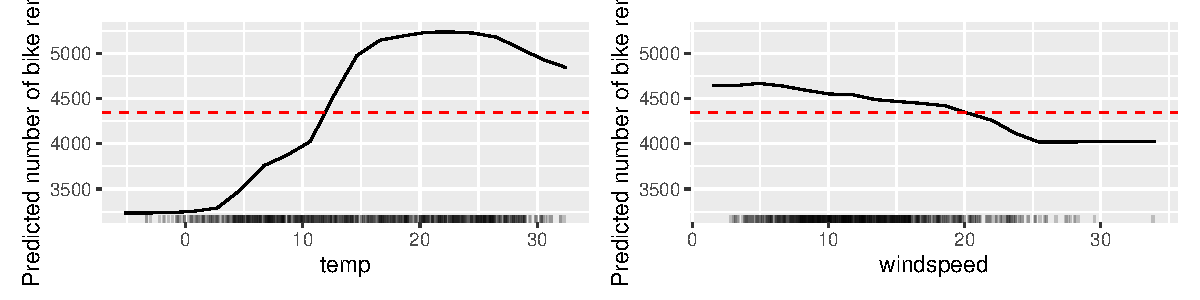
\includegraphics[width=0.5\textwidth]{figure_man/pdps_bike}
\end{center}
\end{frame}

\begin{frame}{PD Feature Importance - Motivation}
\begin{itemize}
    \item The basic motivation is that a flat PDP indicates that the feature is not important
    \item The more the PDP varies, the more important the feature is
\end{itemize}

\begin{center}
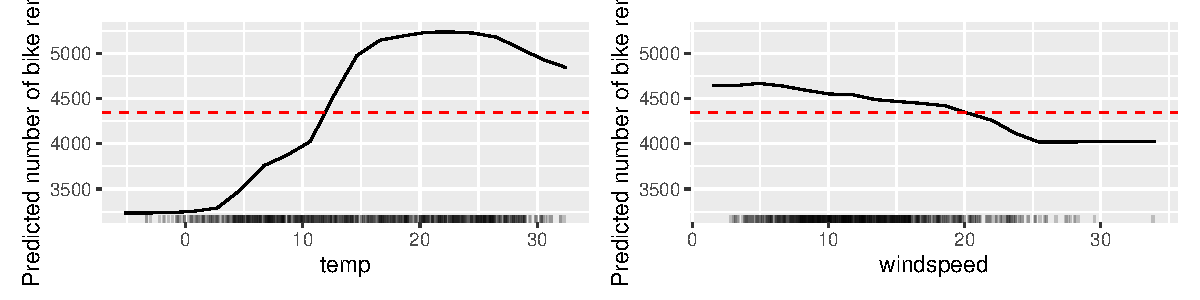
\includegraphics[width=1\textwidth]{figure_man/pdps_bike}
\end{center}

The notion of variable importance is based on any measure of the \textbf{flatness} $\digamma(\cdot)$ of the partial dependence function $\fh$.

$$
I(x)=\digamma\left(\fh_{S}\left(\boldsymbol{z}_{S}\right)\right)
$$

\end{frame}

\begin{frame}{PD Feature Importance - Idea}
\begin{itemize}
    \item Therefore, we focus our attention to the surface that spans between the PDP curve itself and the average of all feature values (red dashed line). $\sum_{k=1}^{K}\hat{f}_{S}\left(x_{S}^{(k)}\right)$
\end{itemize}

\begin{center}
\includegraphics<1>[width=1\textwidth]{figure_man/pdps_bike}
\includegraphics<2>[width=1\textwidth]{figure_man/pdps_dev}
\end{center}


The function $\digamma(\cdot)$ determines the exact quantification of the \textbf{flatness} measure.
\end{frame}

\begin{frame}{Measures of Flatness}
For \textbf{numerical} features, importance is defined as the deviation of each unique feature value from the average curve
$$
I\left(x_{S}\right)=\sqrt{\frac{1}{K-1} \sum_{k=1}^{K}\left(\hat{f}_{S}\left(x_{S}^{(k)}\right)-\frac{1}{K} \sum_{k=1}^{K} \hat{f}_{S}\left(x_{S}^{(k)}\right)\right)^{2}}
$$
\vspace{1cm}

For \textbf{categorical} we achieve a rough estimate of the deviation by applying the range rule: This is the range of the PDP values for the unique categories divided by four.

$$
I\left(x_{S}\right)=\left(\max _{k}\left(\hat{f}_{S}\left(x_{S}^{(k)}\right)\right)-\min _{k}\left(\hat{f}_{S}\left(x_{S}^{(k)}\right)\right)\right) / 4
$$
\end{frame}

\begin{frame}{Discussion}

\textbf{Advantages} \\
variable importance measure that is...
\begin{itemize}
    \item  suitable for use with any supervised learning algorithm, provided new predictions can be obtained
    \item model-based and takes into account the effect of all the features in the model
    \item consistent and has the same interpretation regardless of the learning algorithm employed
    \item has the potential to help identify possible interaction effects.
\end{itemize}

\textbf{Disadvantages} \\
\begin{itemize}
    \item This PDP-based feature importance should be interpreted with care.
    \item It captures only the main effect of the feature and ignores possible feature interactions.
    \item variable importance metric relies on the fitted model; hence, it is crucial to properly tune and train the model to attain the best performance possible.
\end{itemize}
% 
% Disadvantages:  Secondly, 
\end{frame}
\endlecture
\end{document}